% \begin{filecontents}{\jobname.bib}
% @book{Dumke2001,
%     Author = {Dumke},
%     Publisher = {Vieweg},
%     Title = {Software-Engineering},
%     Year = {2001},
%     ISBN = {3-528-25355-X}}
% @book{Balzert1998,
%     Author = {BALZERT, H.},
%     Publisher = {Spektrum Akademischer Verlag},
%     Title = {Lehrbuch der Software-Technik, Band 2: Software-Management, Software-Qualit"atssicherung},
%     Year = {2001},
%     ADDRESS = {Heidelberg; Berlin; Oxford},
%     ISBN = {978-3827400659}}
% \end{filecontents}

% DUMKE (2001): Software-Engineering, Vieweg, ISBN 3-528-25355-X

%%%%%%%%%%%%%%%%%%%%%%%%%%%%%%%%%%%%%%%%%%%%%%%%%%%%%%%%%%%%%%%%%%%%%
% LaTeX Template: Softwaretechnik SS 2017
%
% Date: April 2017
%
%%%%%%%%%%%%%%%%%%%%%%%%%%%%%%%%%%%%%%%%%%%%%%%%%%%%%%%%%%%%%%%%%%%%%%

\documentclass[12pt]{article}
\usepackage[a4paper]{geometry}
\usepackage{framed}
\usepackage[myheadings]{fullpage}
\usepackage{fancyhdr}
\usepackage{lastpage}
\usepackage{graphicx, wrapfig, subcaption, setspace, booktabs}
% \usepackage{movie15}
\usepackage[T1]{fontenc}
\usepackage[font=small, labelfont=bf]{caption}
\usepackage[protrusion=true, expansion=true]{microtype}
\usepackage[ngerman]{babel}
\usepackage[ngerman]{translator}
\usepackage{sectsty}
\usepackage{url, lipsum}
\usepackage[parfill]{parskip}
\usepackage{csquotes}
\usepackage[hidelinks]{hyperref}
\usepackage[acronym]{glossaries}

% \usepackage[utf8]{inputenc}

% \bibliographystyle{numeric}

% \usepackage[style=authoryear,backref=tr"u]{biblatex}
\usepackage[sorting=none,backref=true, backend=biber]{biblatex}
\addbibresource{\jobname.bib}
% \usepackage[numbers,round]{natbib}
% \AtEveryCitekey{\clearfield{url}\clearfield{doi}\clearfield{isbn}\clearfield{issn}}


\usepackage[export]{adjustbox}
\usepackage{multicol}
\usepackage{tikz}
\usepackage{float}

\usepackage{pdfpages}


\makeglossaries
\glstoctrue



%-------------------------------------------------------------------------------
% Commands
%-------------------------------------------------------------------------------
\newcommand{\HRule}[1]{\rule{\linewidth}{#1}}
\input{../../env}
%-------------------------------------------------------------------------------
% HEADER & FOOTER
%-------------------------------------------------------------------------------
\fancypagestyle{myplain}
{
\fancyhf{}
\paperwidth=\pdfpageheight
\paperheight=\pdfpagewidth
\pdfpageheight=\paperheight
\pdfpagewidth=\paperwidth
\headwidth=\textwidth
\renewcommand\headrulewidth{0pt}
\renewcommand\footrulewidth{0pt}
\fancyfoot[R]{Seite \thepage\ von \pageref{LastPage}}

}

\fancypagestyle{myfancy}{
  \fancyhf{}
  \pagestyle{fancy}
  \fancyhf{}
  \setlength\headheight{15pt}
  \fancyhead[L]{\newCommandName}
  \fancyhead[R]{\newCommandUniversity}
  \fancyfoot[R]{Seite \thepage\ von \pageref{LastPage}}
}
% \pagestyle{fancy}
% \fancyhf{}
% \setlength\headheight{15pt}
% \fancyhead[L]{\newCommandName}
% \fancyhead[R]{\newCommandUniversity}
% \fancyfoot[R]{Seite \thepage\ von \pageref{LastPage}}

%-------------------------------------------------------------------------------
% TITLE PAGE
%-------------------------------------------------------------------------------
\begin{document}
\hypersetup{
    % colorlinks,
    citecolor=black,
    filecolor=black,
    linkcolor=black,
    urlcolor=black
}


\title{ \normalsize
		\HRule{0.5pt} \\
		\LARGE \textbf{\uppercase{\newCommandDiscipline}} \\
    \smallbreak
		% \small\textbf{{\newCommandTerm}}\\
    % \small\textbf{{\newCommandKind}}\\
    \small\textbf{{UML - Unified Modeling Language}}\\
		\HRule{2pt} \\ [0.5cm]
    \small\textbf{{\newCommandTerm}}\\
    [0.5cm]
    \normalsize \today \vspace*{10\baselineskip}}

\date{}



\author{
    \newCommandName \\
		\newCommandMatriculationNumber \\
		\newCommandUniversity \\
		\newCommandFaculty
}

% \pagenumbering{gobble}

\maketitle
\thispagestyle{empty}

\newpage

\thispagestyle{myfancy}
\tableofcontents
% \listoffigures
\newpage



%-------------------------------------------------------------------------------
% Section title formatting
\sectionfont{\scshape}
%-------------------------------------------------------------------------------

%-------------------------------------------------------------------------------
% BODY
%-------------------------------------------------------------------------------

% \section{SWT - Einf"uhrung in die Softwaretechnik}
% \thispagestyle{myplain}

% \thispagestyle{beamer}

% 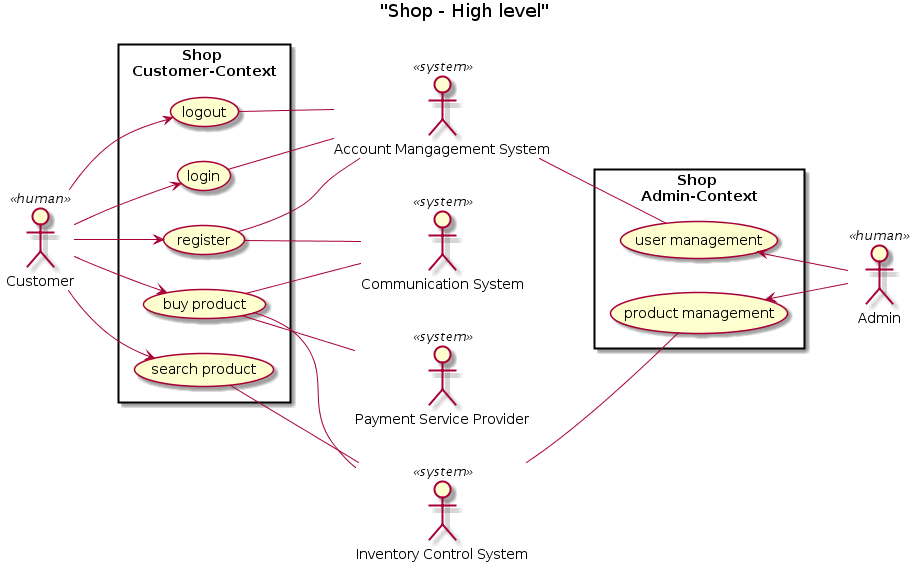
\includepdf[landscape,pages=1,addtotoc={1, section, 1,``heading'', ``label''}]{./pdf/01_use_case_shop}
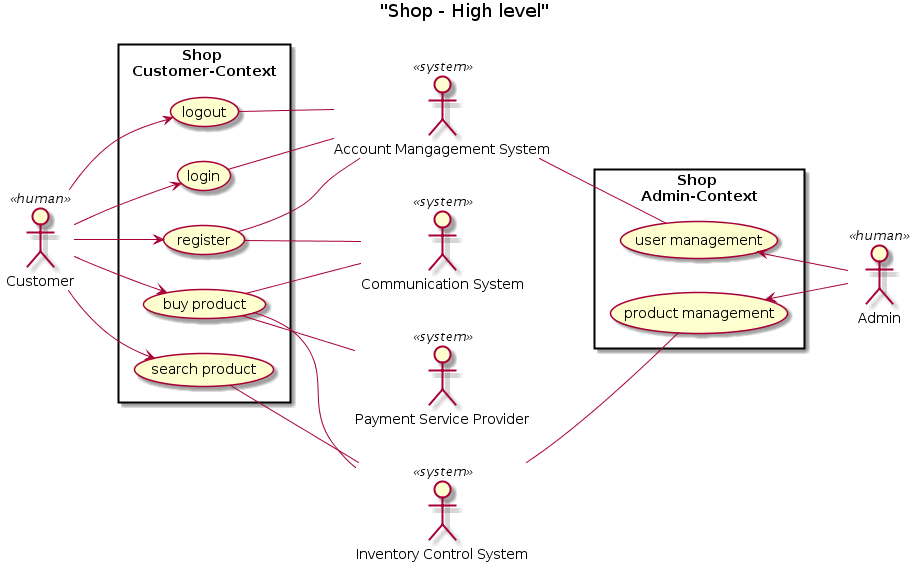
\includepdf[landscape,pages=1,addtotoc={
     1,section,1,Use-Case-Diagram,p1,
     1,subsection,1,High Level,p2
     }]{./pdf/01_use_case_shop}
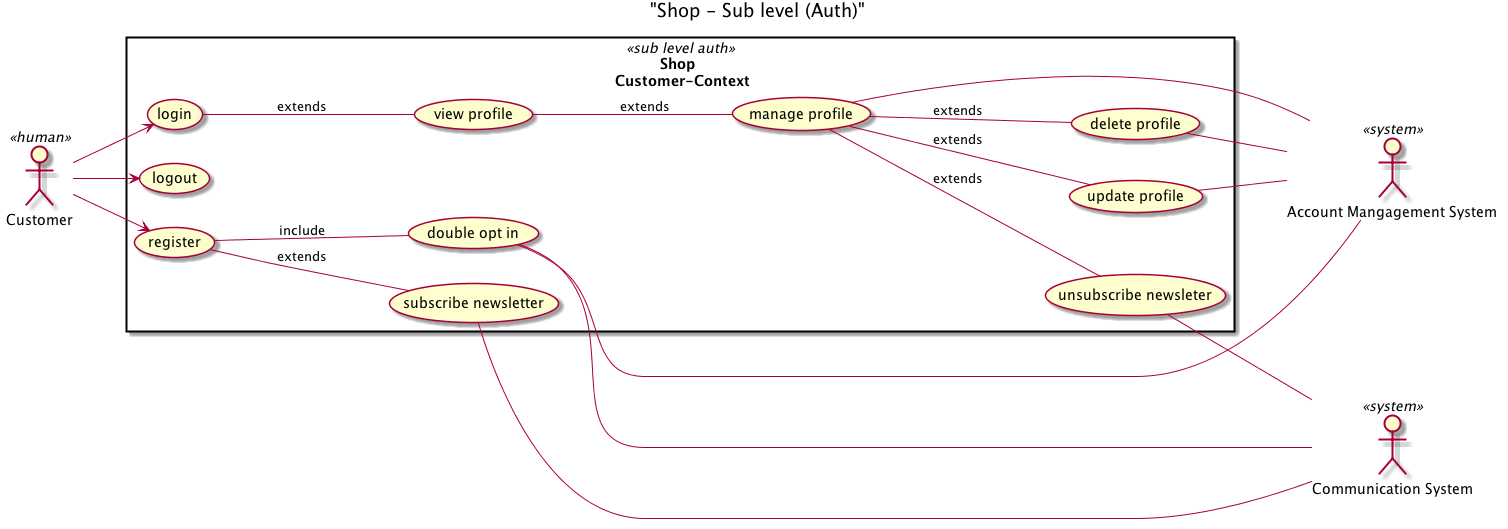
\includepdf[landscape,pages=1,addtotoc={
    %  1,section,1,UML-Diagram,p1,
     1,subsection,1,Sub Level (Auth),p2
     }]{./pdf/02_use_case_shop}
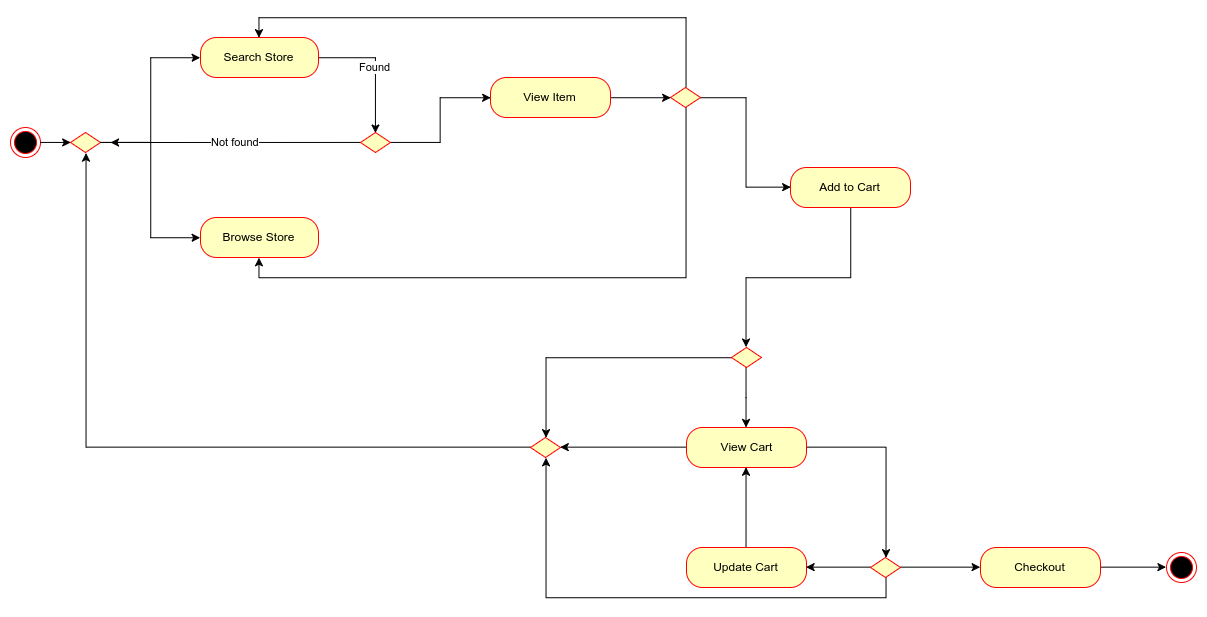
\includepdf[landscape,pages=1,addtotoc={
     1,section,1,Activity-Diagram,p1,
     1,subsection,1,Find Product,p2
     }]{./pdf/03_activity.pdf}
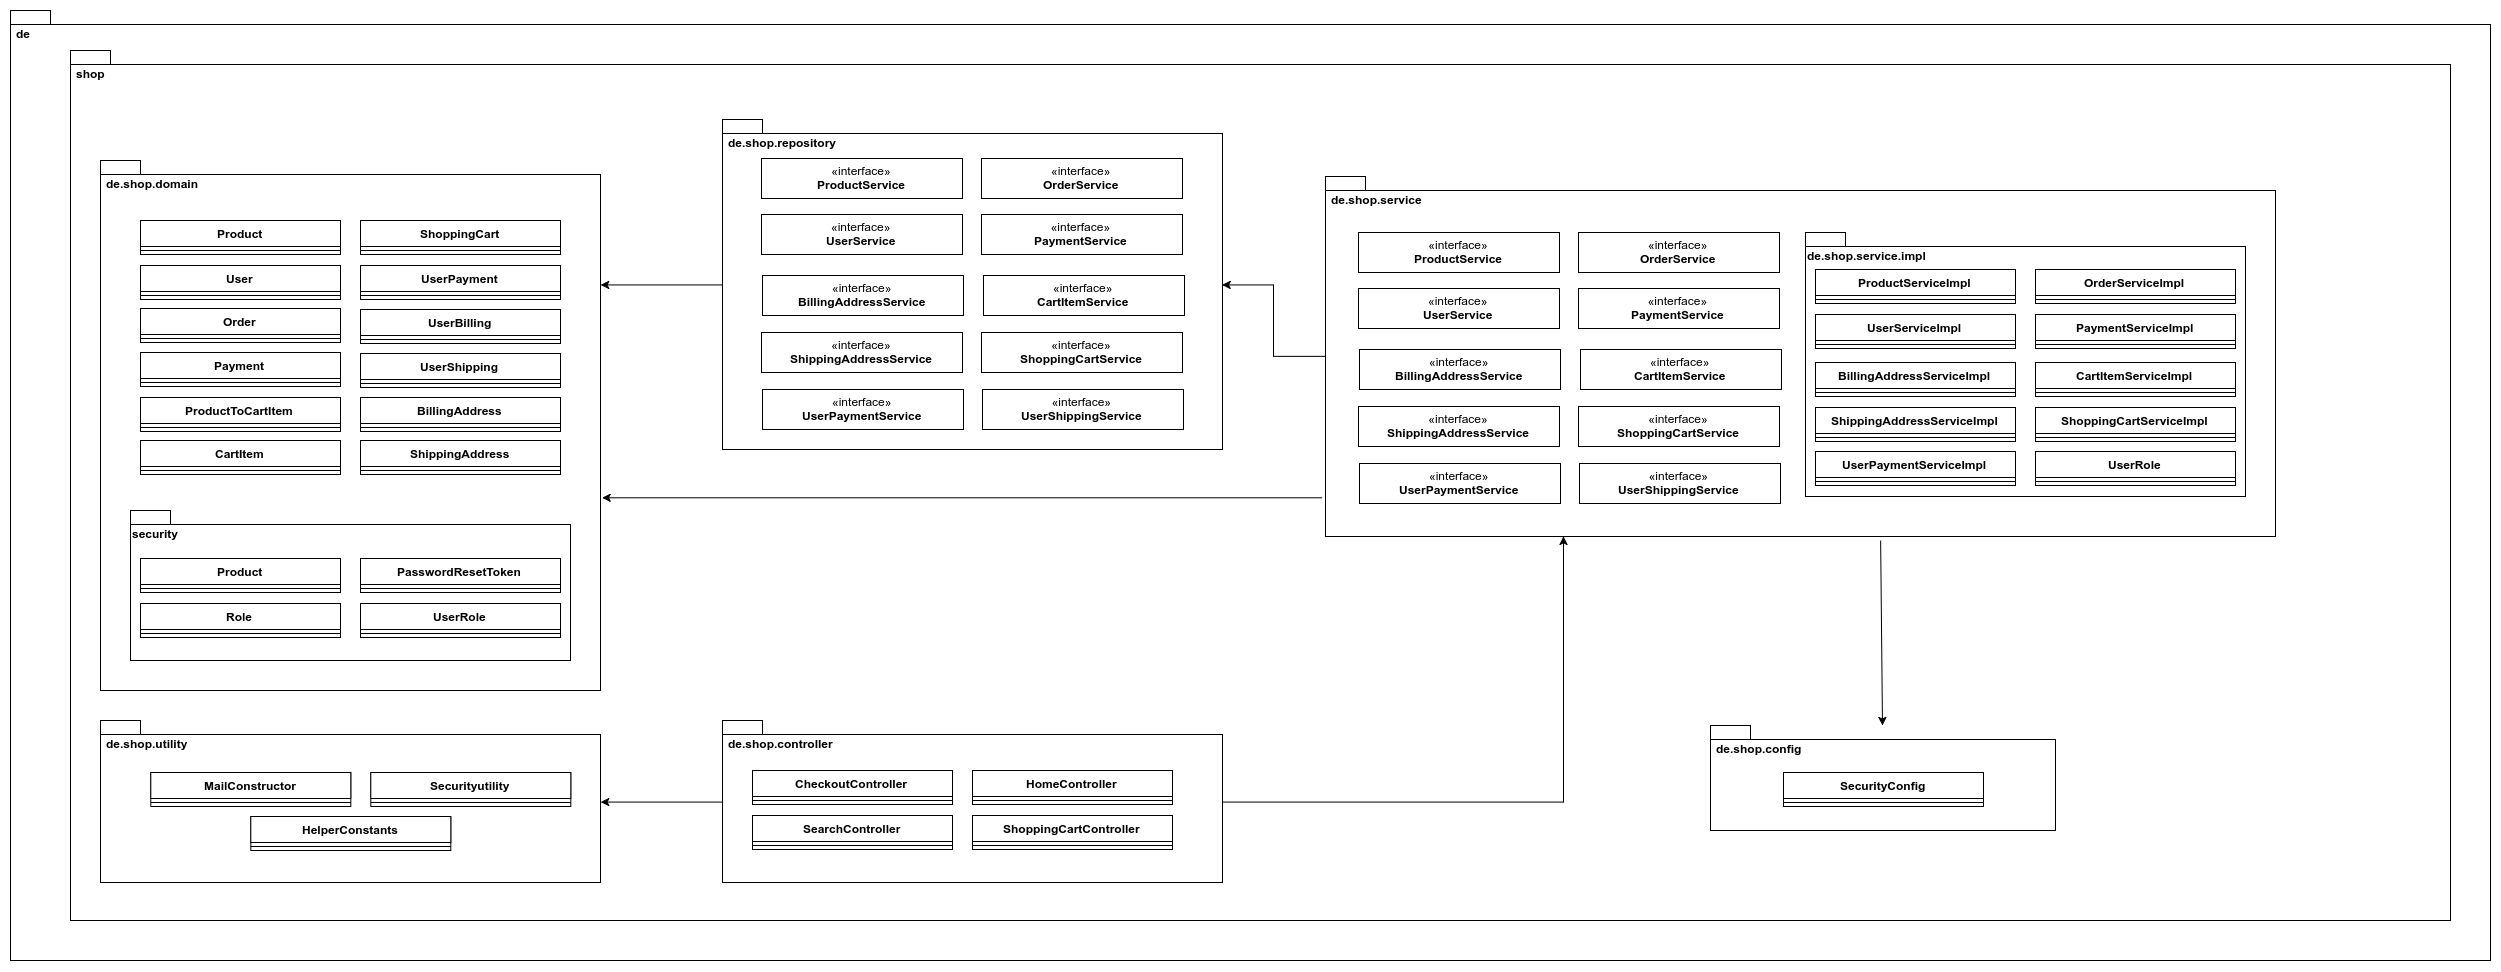
\includepdf[landscape,pages=1,addtotoc={
     1,section,1,Package-Diagram,p1,
     1,subsection,1,Package Productstore,p2
     }]{./pdf/04_package.pdf}
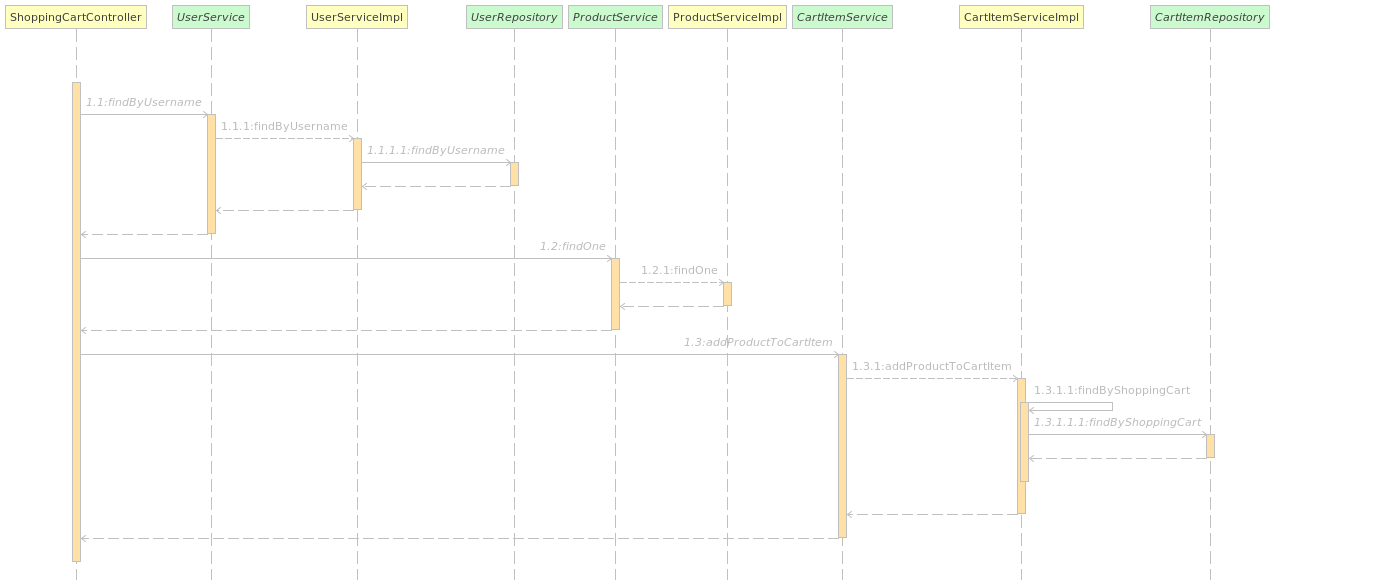
\includepdf[landscape,pages=1,addtotoc={
     1,section,1,Sequence-Diagramm,p1,
     1,subsection,1,Add Item to Cart,p2
     }]{./pdf/05_addItemToCart_sequence.pdf}
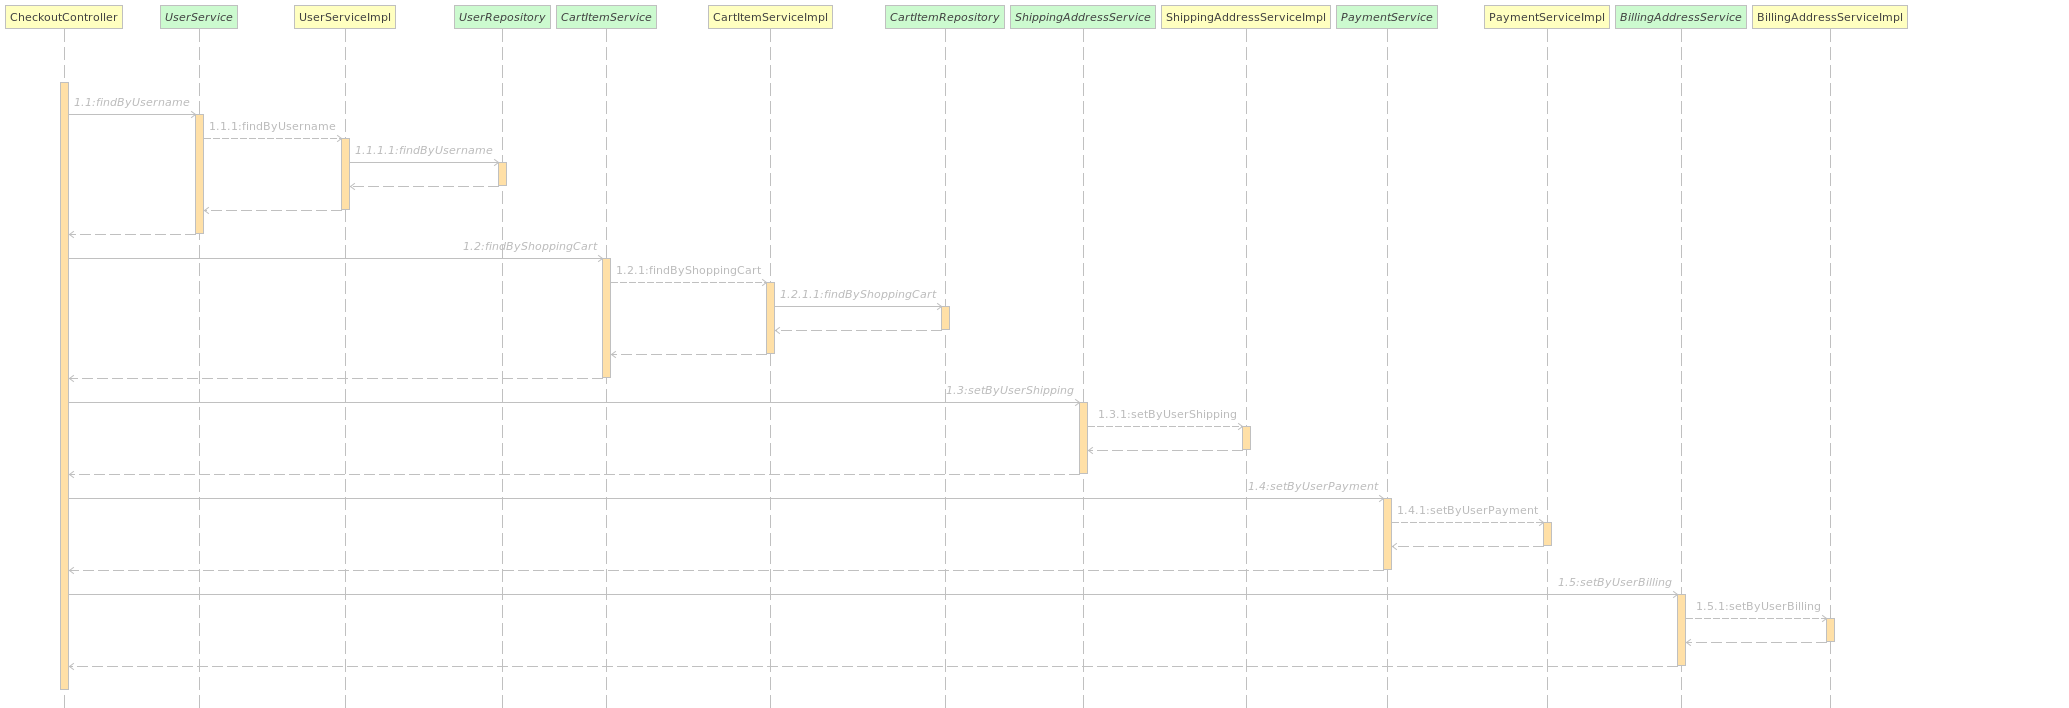
\includepdf[landscape,pages=1,addtotoc={
    %  1,section,1,Sequence-Diagramm,p1,
     1,subsection,1,Checkout,p2
     }]{./pdf/06_checkout_sequence.pdf}
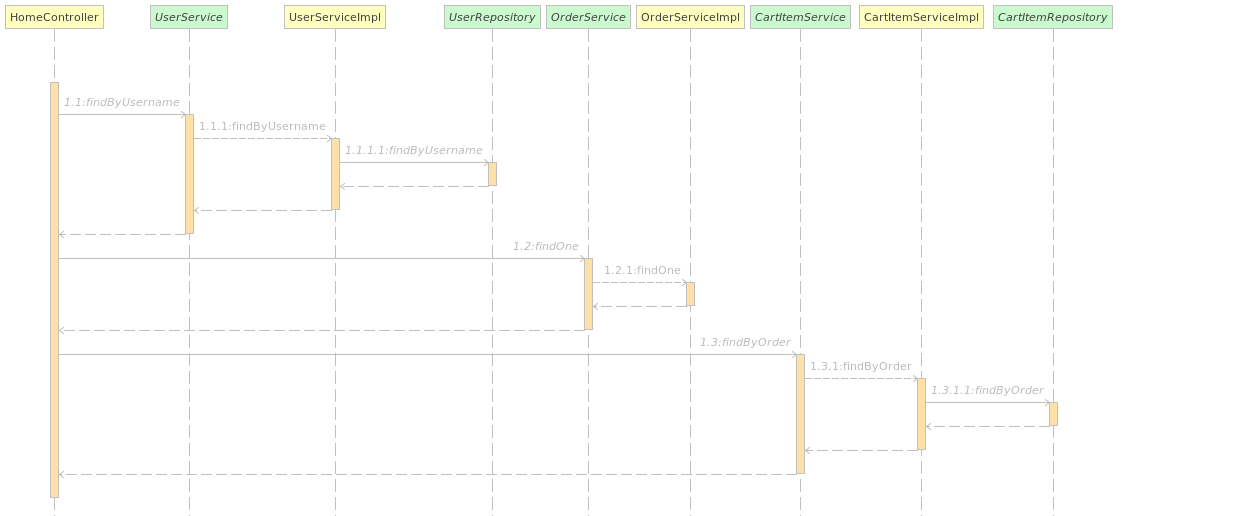
\includepdf[landscape,pages=1,addtotoc={
    %  1,section,1,Sequence-Diagramm,p1,
     1,subsection,1,Order Detail History,p2
     }]{./pdf/07_orderDetailHistory_sequence.pdf}
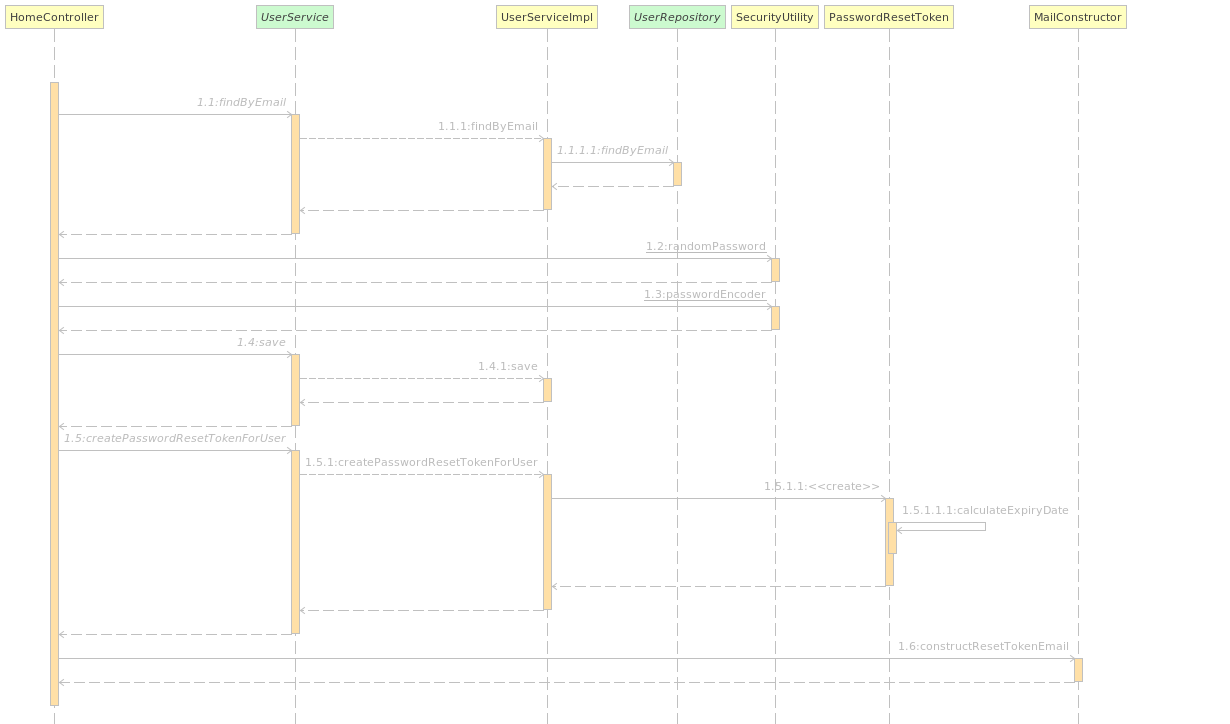
\includepdf[landscape,pages=1,addtotoc={
    %  1,section,1,Sequence-Diagramm,p1,
     1,subsection,1,Password-Reset,p2
     }]{./pdf/08_passwordReset_sequence.pdf}
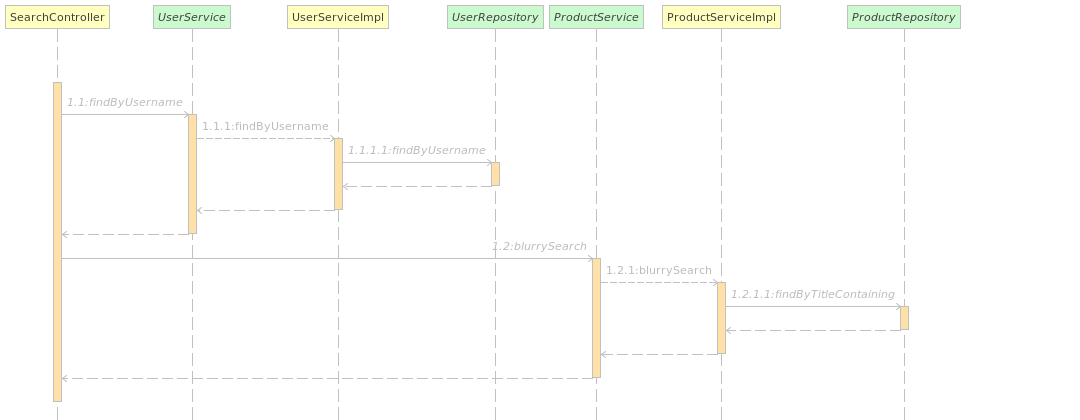
\includepdf[landscape,pages=1,addtotoc={
    %  1,section,1,Sequence-Diagramm,p1,
     1,subsection,1,Search Product,p2
     }]{./pdf/09_searchProduct_sequence.pdf}
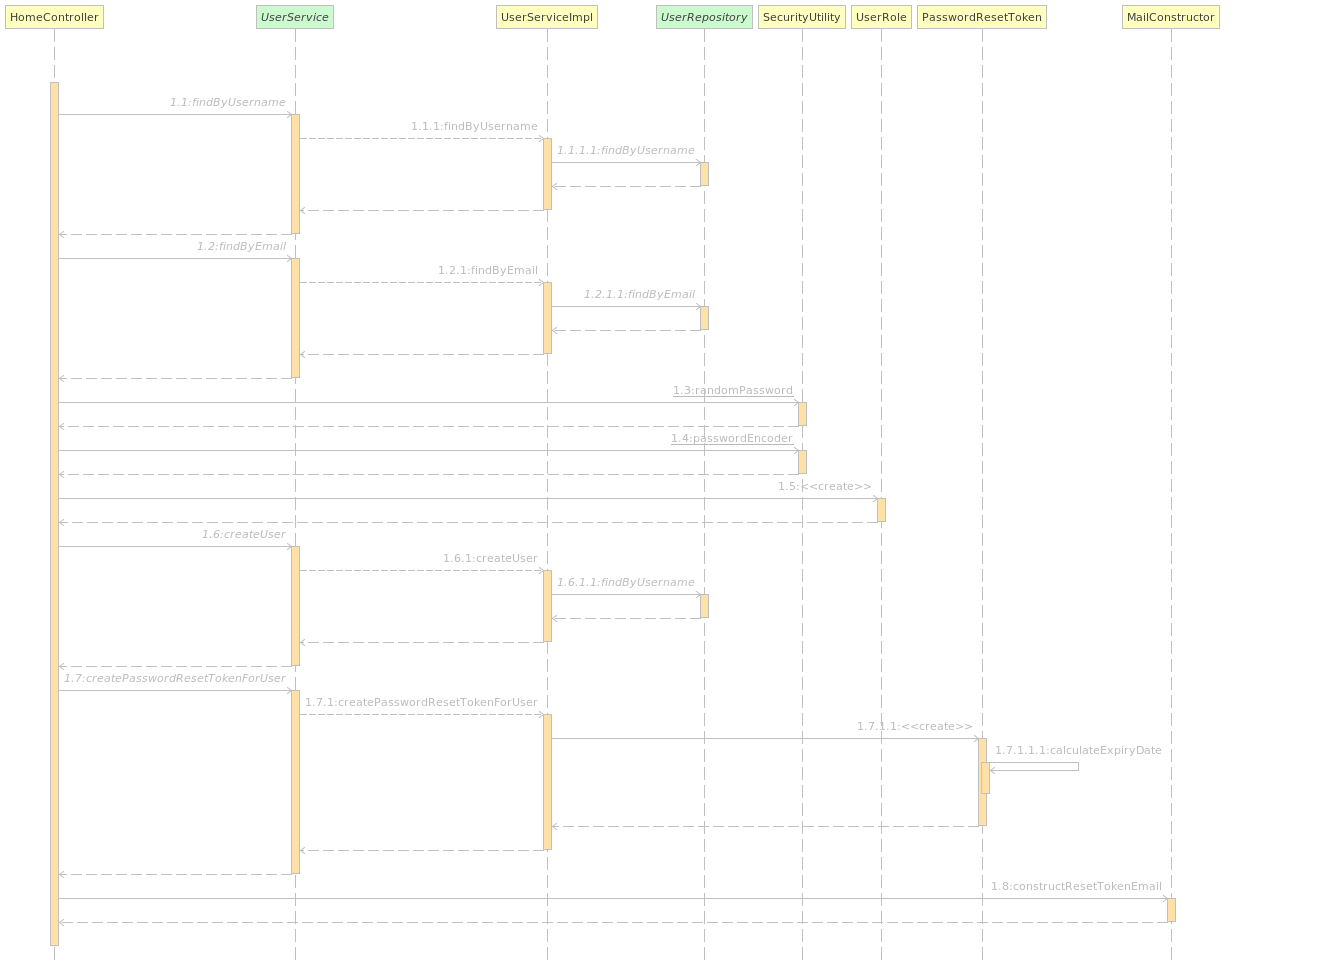
\includepdf[landscape,pages=1,addtotoc={
    %  1,section,1,Sequence-Diagramm,p1,
     1,subsection,1,User-Registration,p2
     }]{./pdf/10_userRegistration_sequence.pdf}
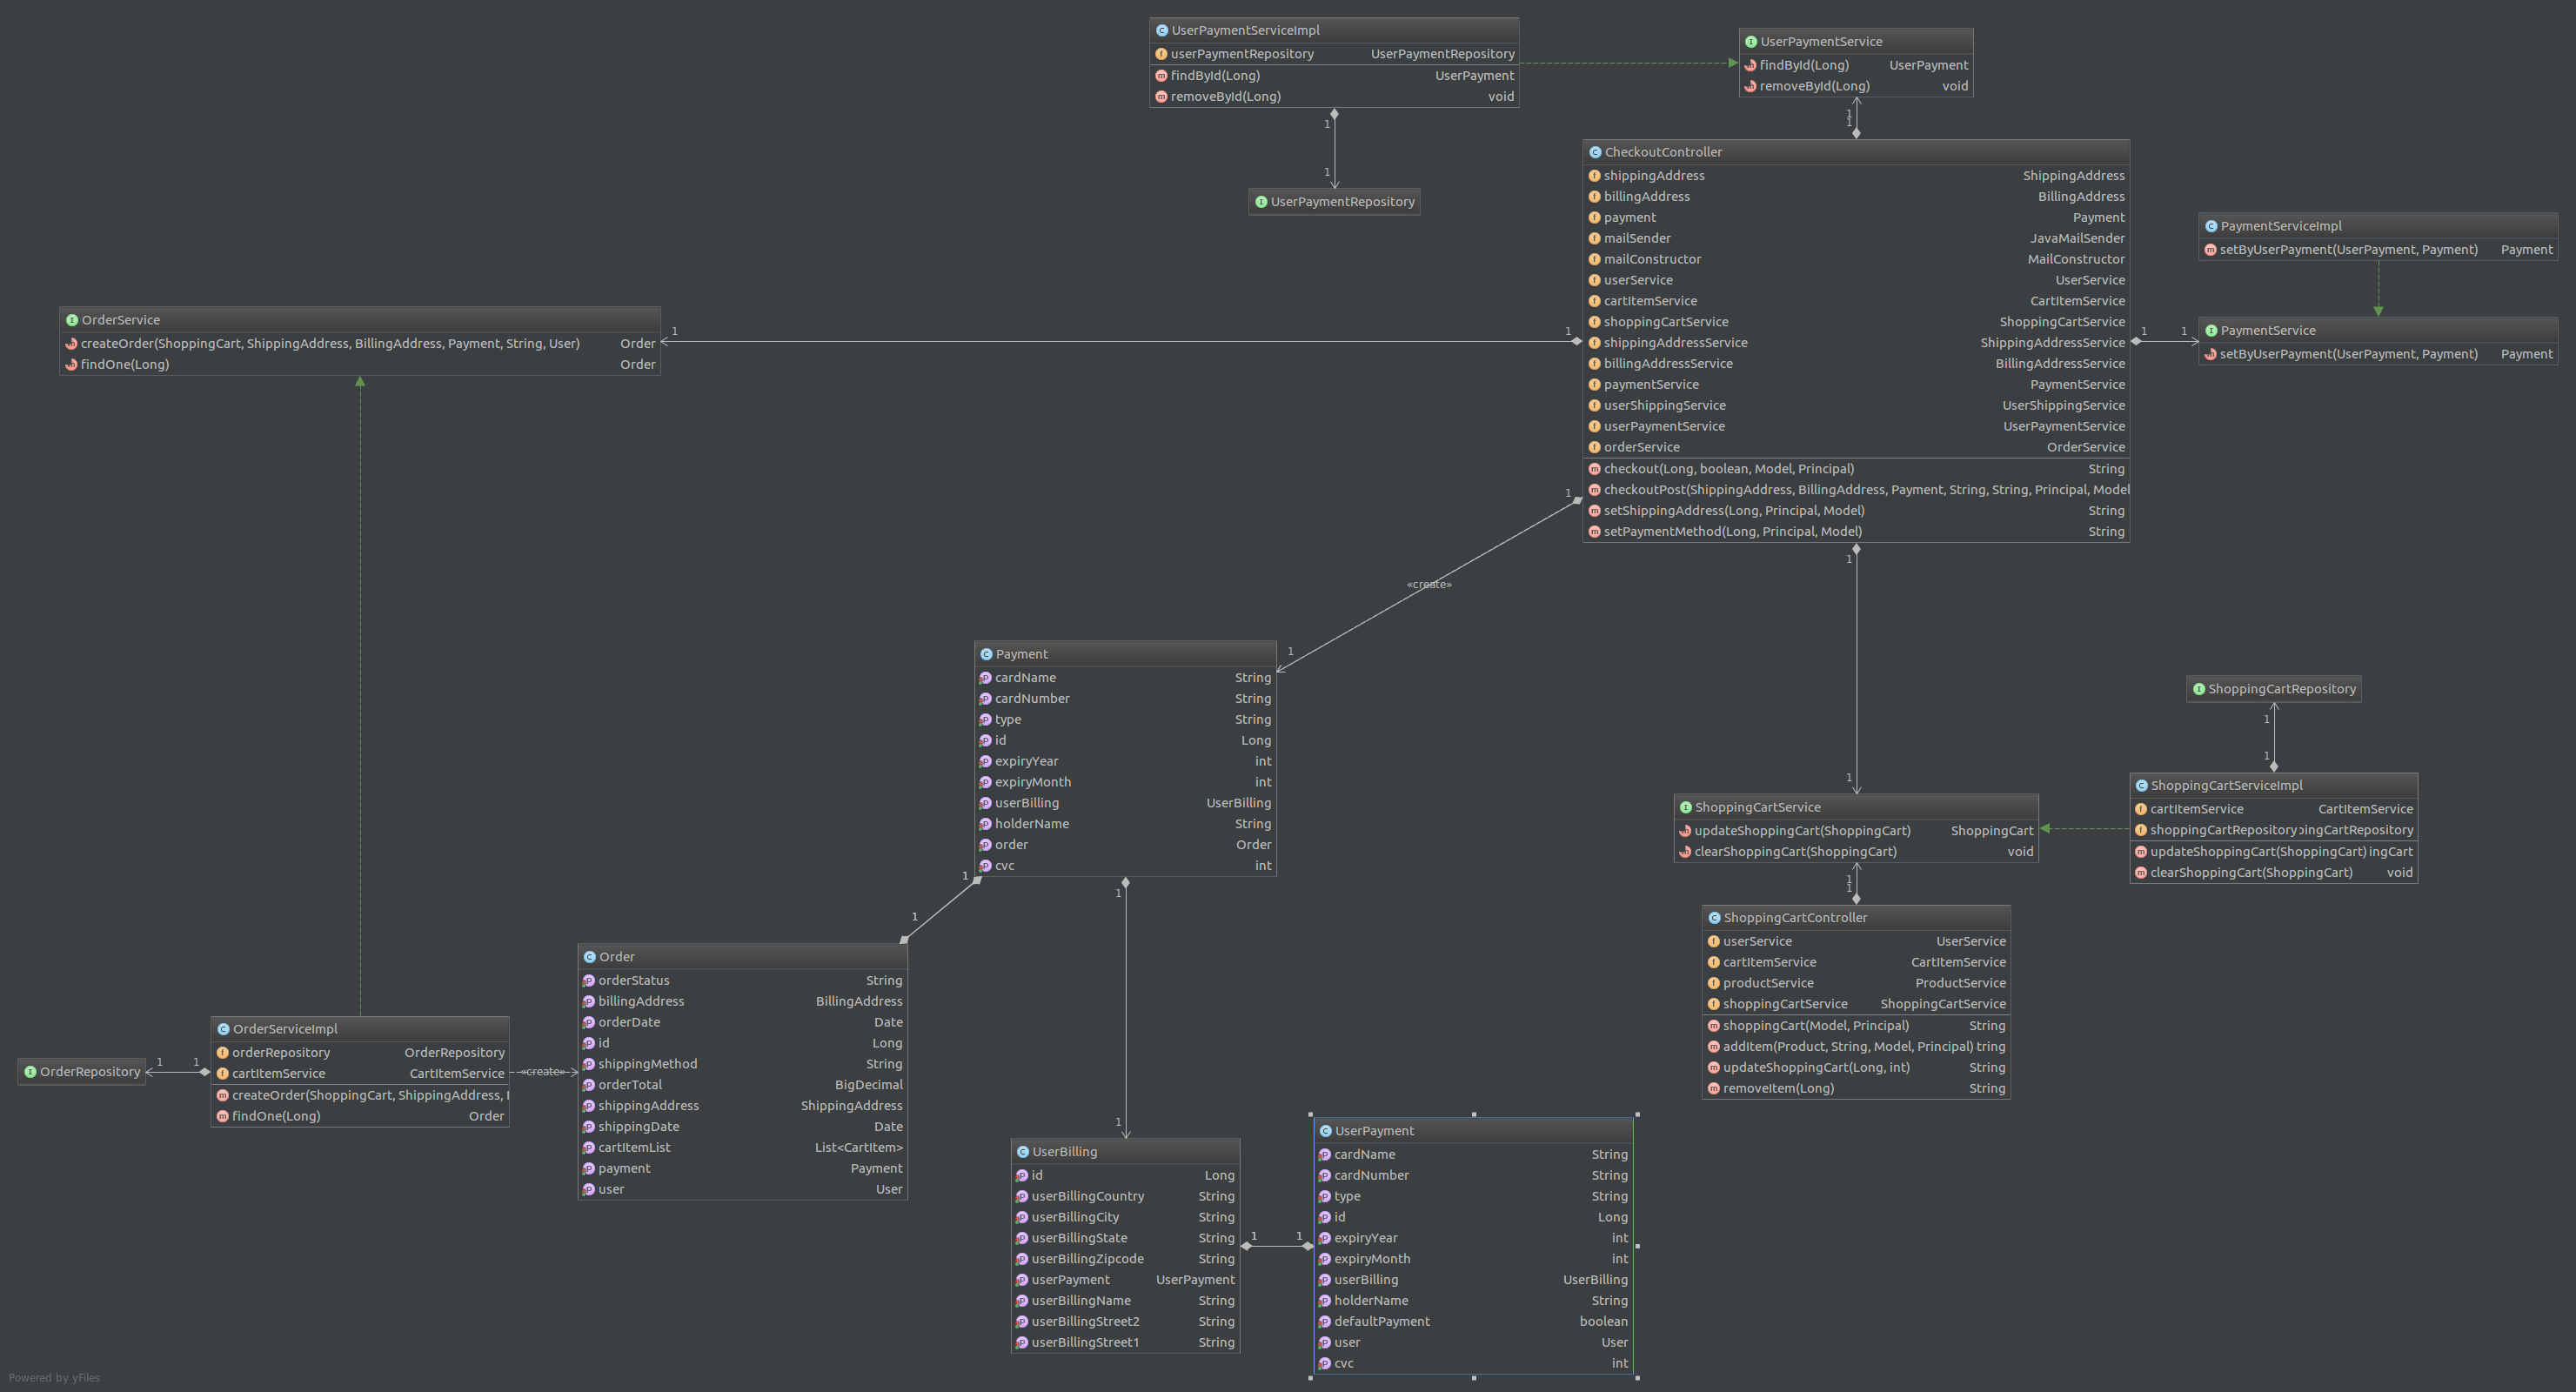
\includepdf[landscape,pages=1,addtotoc={
     1,section,1,Class-Diagramm,p1,
     1,subsection,1,Checkout-Order,p2
     }]{./pdf/11_checkoutOrder.pdf}
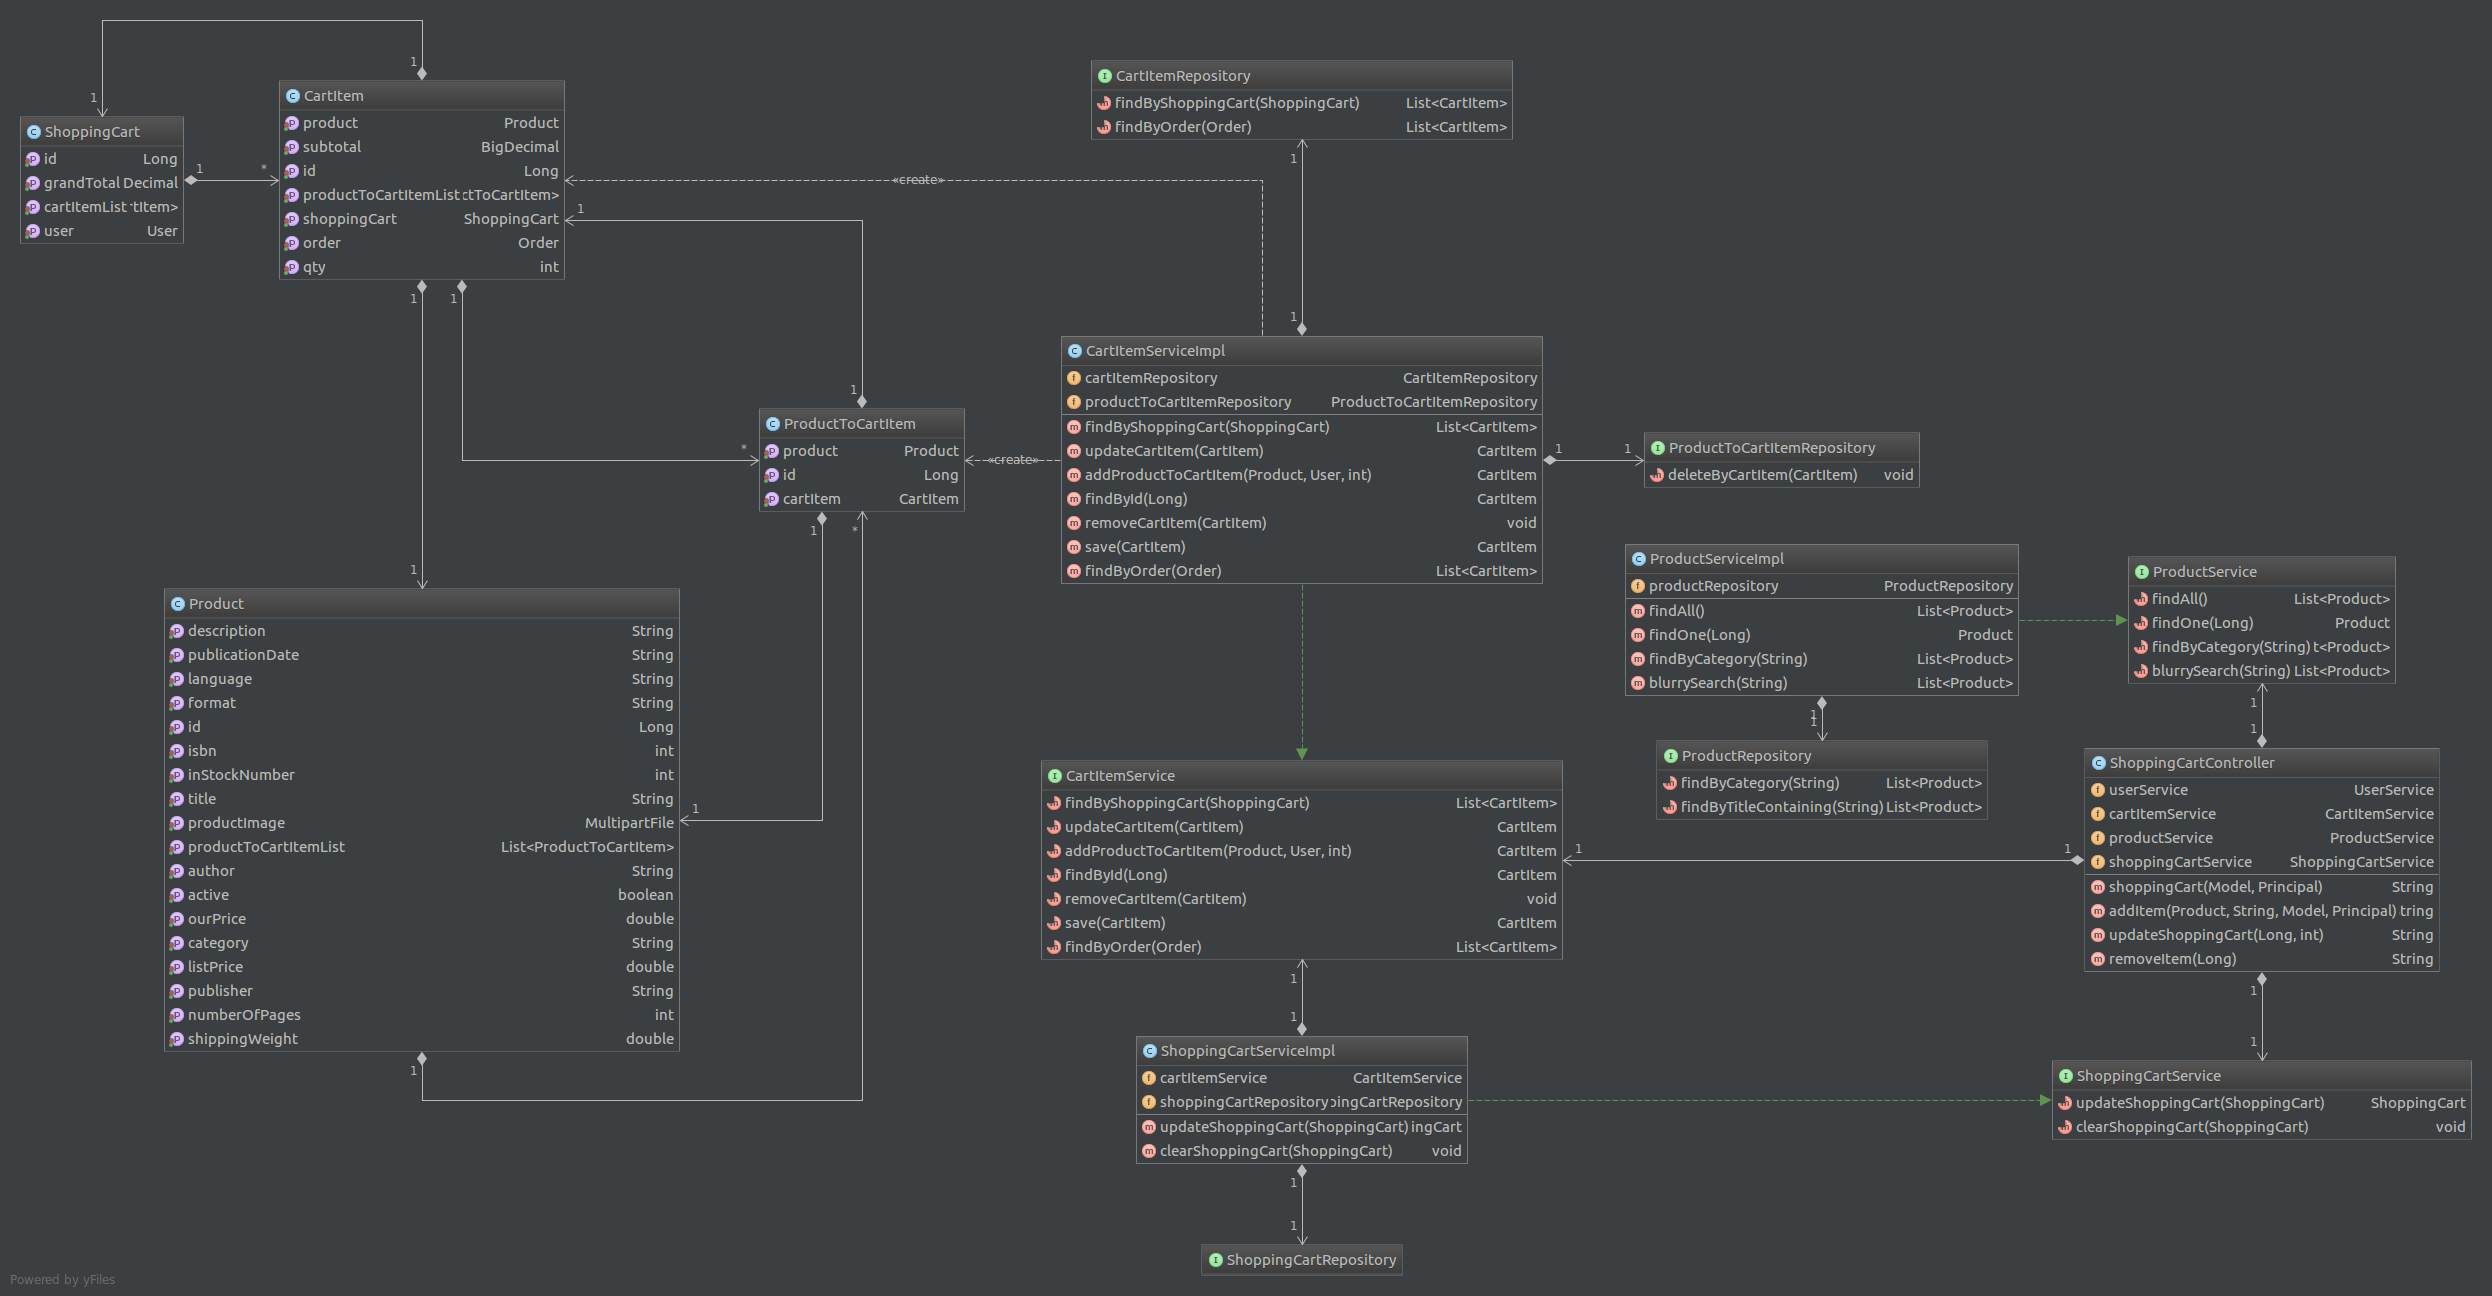
\includepdf[landscape,pages=1,addtotoc={
    %  1,section,1,Class-Diagramm,p1,
     1,subsection,1,Product-Shopping-Cart,p2
     }]{./pdf/12_ProductShoppingCart.pdf}
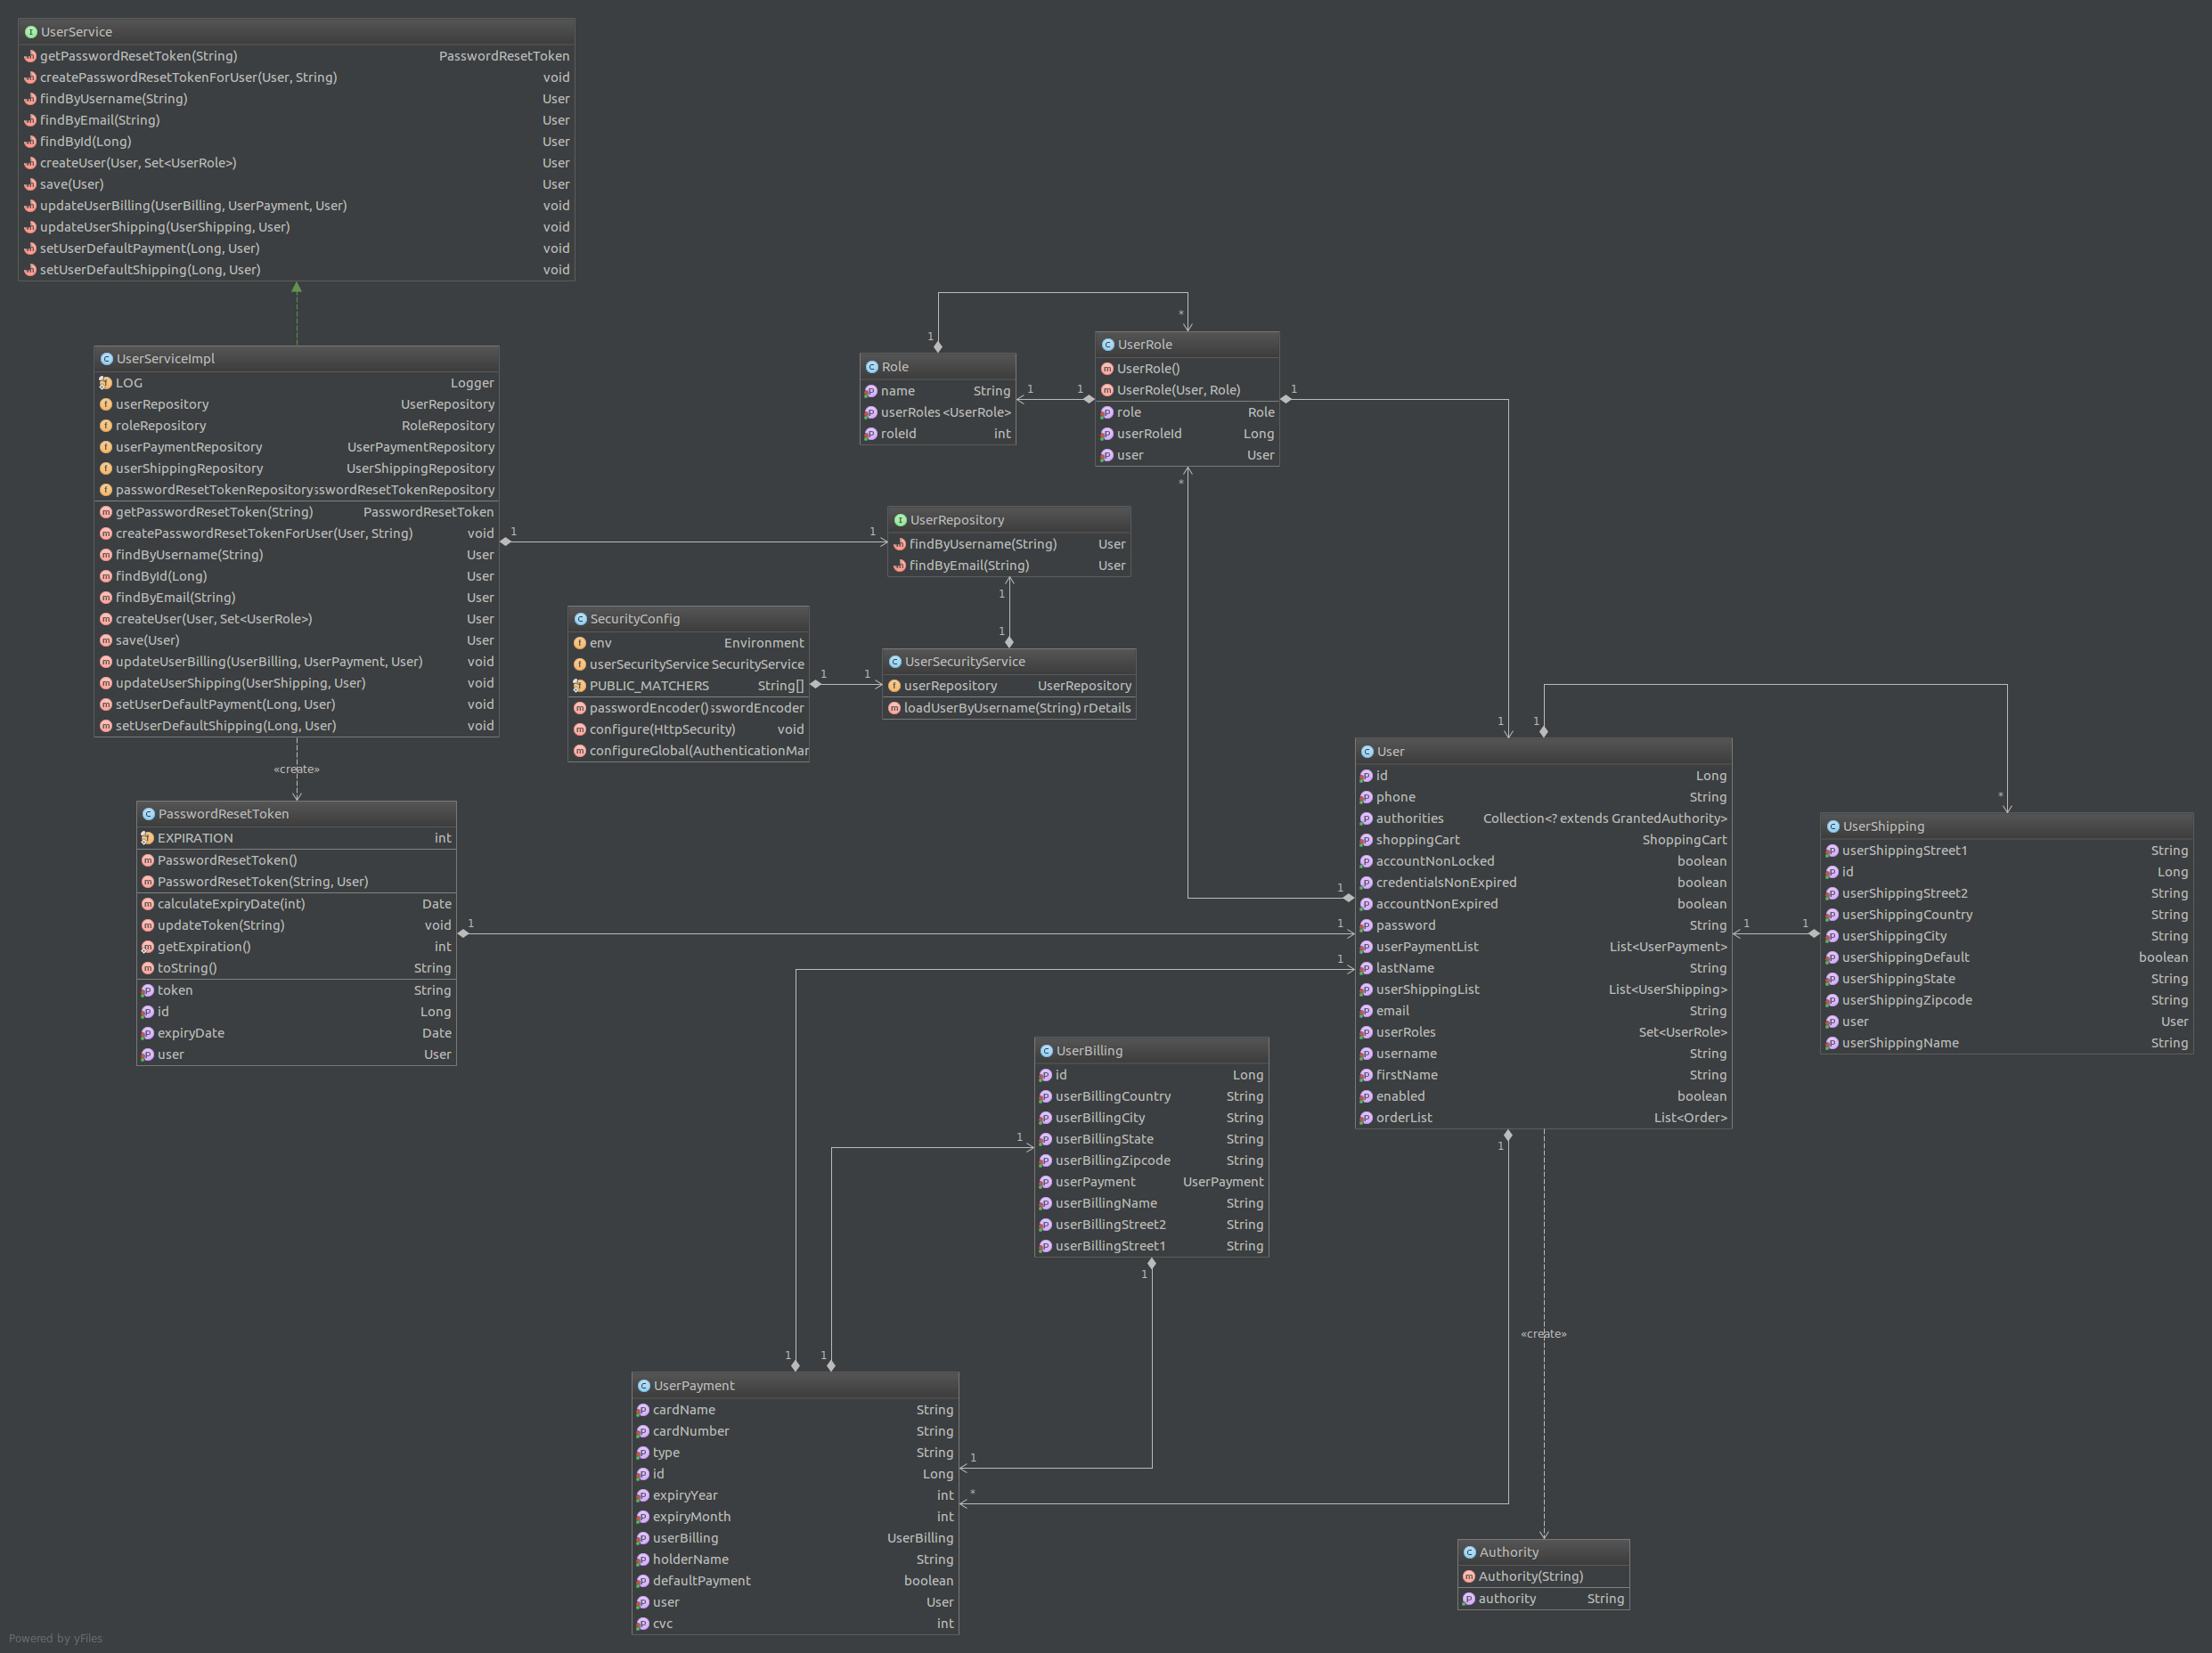
\includepdf[landscape,pages=1,addtotoc={
    %  1,section,1,Class-Diagramm,p1,
     1,subsection,1,Customer,p2
     }]{./pdf/13_user.pdf}

% 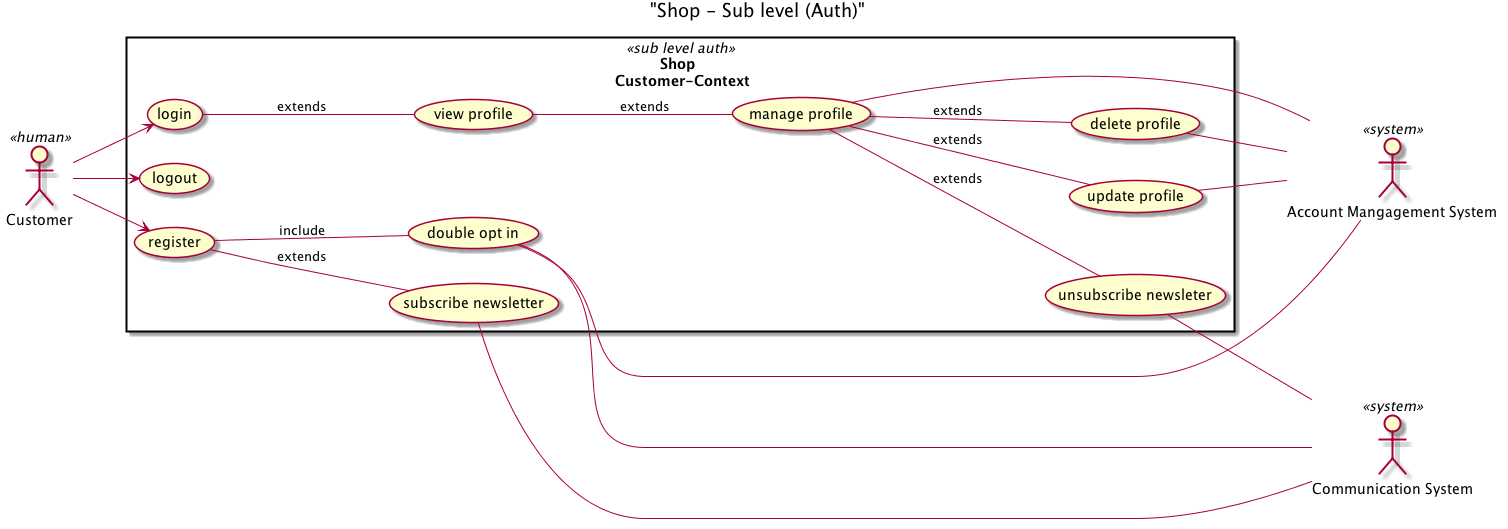
\includepdf[fitpaper=true,pages=1,addtotoc={1, section, 2,``heading'', ``label''}]{./pdf/02_use_case_shop}


% 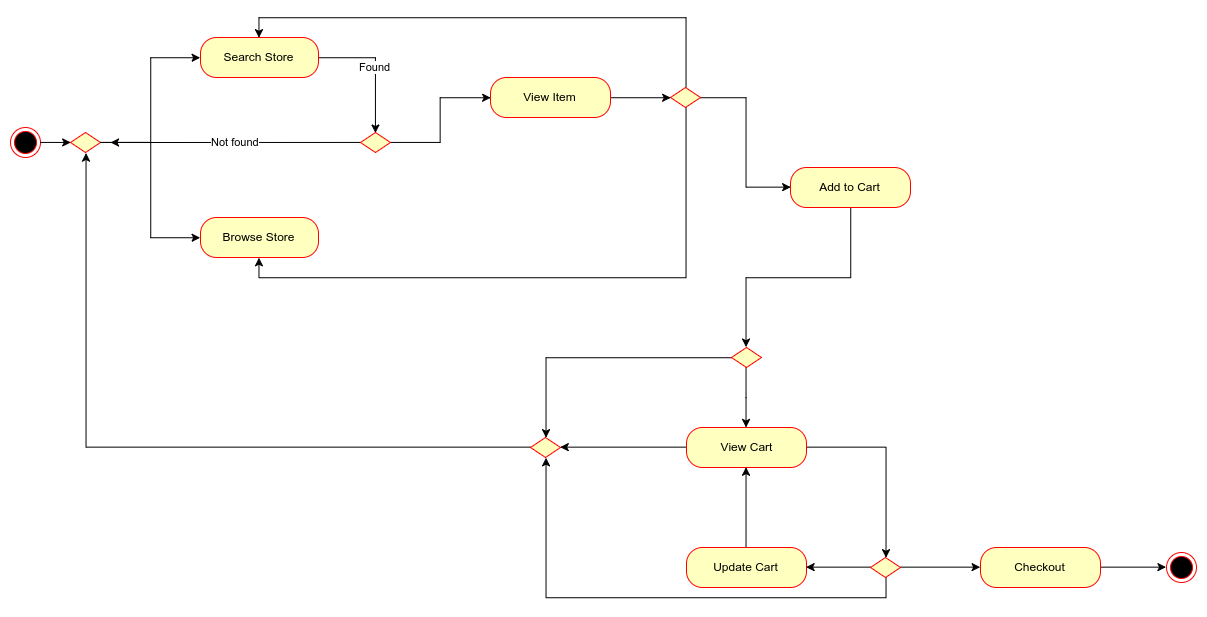
\includepdf[fitpaper=true,pages=1,addtotoc={1, section, 3,``heading'', ``label''}]{./pdf/03_activity.pdf}

%-------------------------------------------------------------------------------
% #1
%-------------------------------------------------------------------------------










%-------------------------------------------------------------------------------
% Literatur - Glossar - Akronyme
%-------------------------------------------------------------------------------

% \clearpage
% \setlength\bibitemsep{10pt}
% \printbibliography[heading=bibintoc]
% \newpage
% \printglossary[type=main,title=Glossar]
% \printglossary[type=\acronymtype, title=Akronyme]


%-------------------------------------------------------------------------------
% ENDE
%-------------------------------------------------------------------------------

\end{document}
